
% Opisowy model stanu istniejącego
% Opis wszystkich składników organizacyjnych
% Związek struktury z dziedziną obszaru modelowania, wyznaczenie zakresu odpowiedzialności systemu 	

\textbf{Grupa Kapitałowa Biosystem} składa się z trzech podmiotów gospodarczych (\textbf{BIOSYSTEM S.A.}, \textbf{BIOSYSTEM ElektrorecyklingOrganizacja Odzysku Sprzętu Elektrycznego i Elektronicznego S.A.}, \textbf{Zakład Gospodarki Komunalnej Organizacja Odzysku BIOSYSTEM S.A.}. Firma \textbf{BIOSYSTEM S.A.} stanowi spółkę nadrzędną.

\begin{figure}[H]
	\centering
	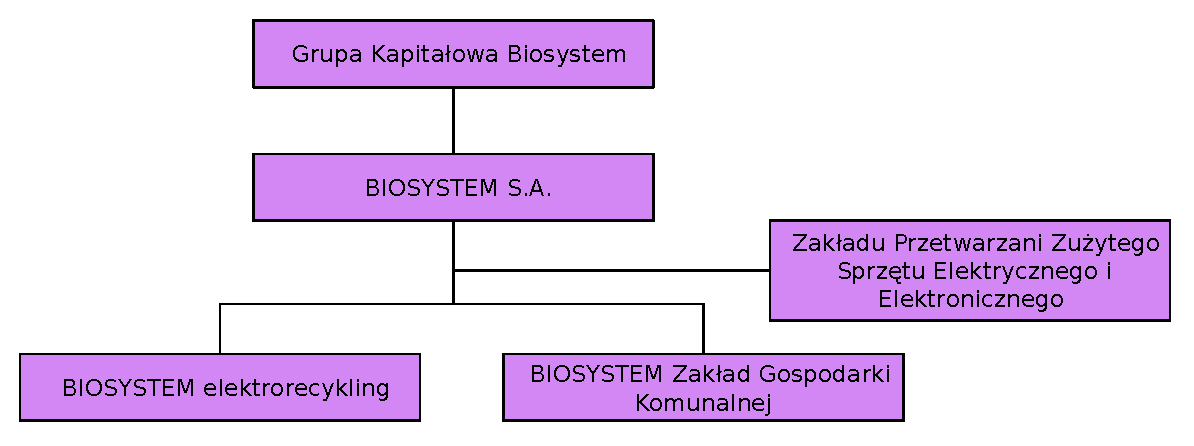
\includegraphics[width=\textwidth]{img/group_chart.eps}
	\caption{Struktura grupy kapitałowej}
\end{figure}


\begin{figure}[H]
    \centering
    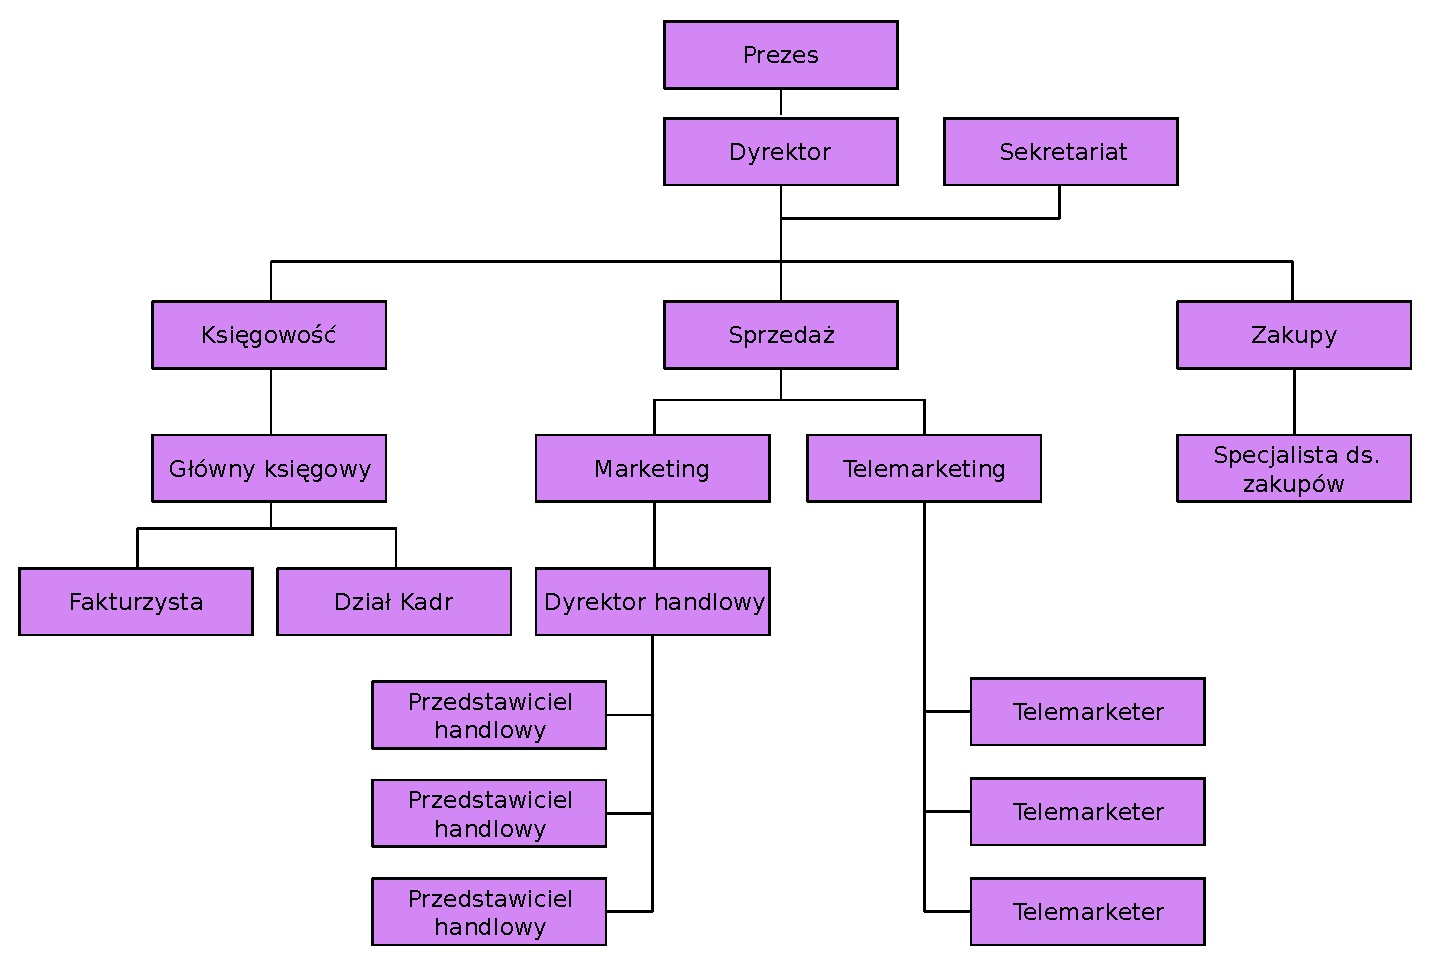
\includegraphics[width=1\textwidth]{img/organization_chart.eps}
    \caption{Struktura organizacyjna spółki}
\end{figure}